\documentclass[a4paper]{article}

\usepackage{mathrsfs}
% ============================================
%         General Packages
% ============================================
\usepackage{balance}

\usepackage{kotex}      % for Korean
\usepackage{lipsum}     % for dummy text
\usepackage{array}

\usepackage{cite}   % for citation

\usepackage{amsmath,amsfonts}
\usepackage{amssymb}
\usepackage{soul}
\usepackage{mathrsfs}

\usepackage{hyperref}

    \hypersetup{
        pdftoolbar=false,        	% show Acrobat’s toolbar?
        pdfmenubar=false,        	% show Acrobat’s menu?
        pdffitwindow=false,     	% window fit to page when opened
        pdfstartview={FitH},    	% fits the width of the page to the window
        pdftitle={},    	% title
        pdfauthor={},     	% author
        %     pdfsubject={},   	% subject of the document
        %     pdfcreator={},   	% creator of the document
        %     pdfproducer={}, 	% producer of the document
        %     pdfkeywords={keyword1, key2, key3}, % list of keywords
        %     pdfnewwindow=true,      	% links in new PDF window
        colorlinks=true,       	% false: boxed links; true: colored links
        linkcolor=blue,          	% color of internal links (change box color with linkbordercolor)
        citecolor=blue,       	% color of links to bibliography
        filecolor=blue,      	% color of file links
        urlcolor=blue		% color of external links
    }

\usepackage{algorithm}
\usepackage{algorithmic}

\usepackage{epsfig}
\usepackage[dvipsnames]{xcolor}

% MY PACKAGES ===================================

\usepackage{svg}
\usepackage{subfig}

\usepackage{textcomp}
\usepackage{stfloats}
\usepackage{url}
\usepackage{verbatim}
\usepackage{graphicx}
\usepackage{multirow}
\usepackage{multicol}

\let\proof\relax
\let\endproof\relax
\usepackage{amsthm}
\usepackage{lipsum}
\usepackage{tikz}

% 
\usepackage{titlepic}
\usepackage{pdfpages}
\usepackage{etoolbox} % 조건문을 쓰기 위한 패키지


\titlepic{%
  
\includegraphics[height = 8mm]{figures/logo_KAIST_simple.png}
  \hspace{5mm}
  
\includegraphics[height = 8mm]{figures/MIC_Logo.png}
  }

% ========================================
%         TITLE and AUTHORS
% ========================================
\title{
  Structured Critic Adaptation
}

\author{
    Soobin Hwang
    \thanks{\href{https://kaist-mic-lab.github.io/members/sbHwang/}{Soobin Hwang} is Integrated M.S./Ph.D. student at KAIST, {\tt\small tnqls2361@kaist.ac.kr}}%
}

\date{
    % 20\textsuperscript{th} March 2025
    Complied on \today
}

\begin{document}

\maketitle

% ========================================
%         Contents
% ========================================

\begin{figure}[h]
  \centering
  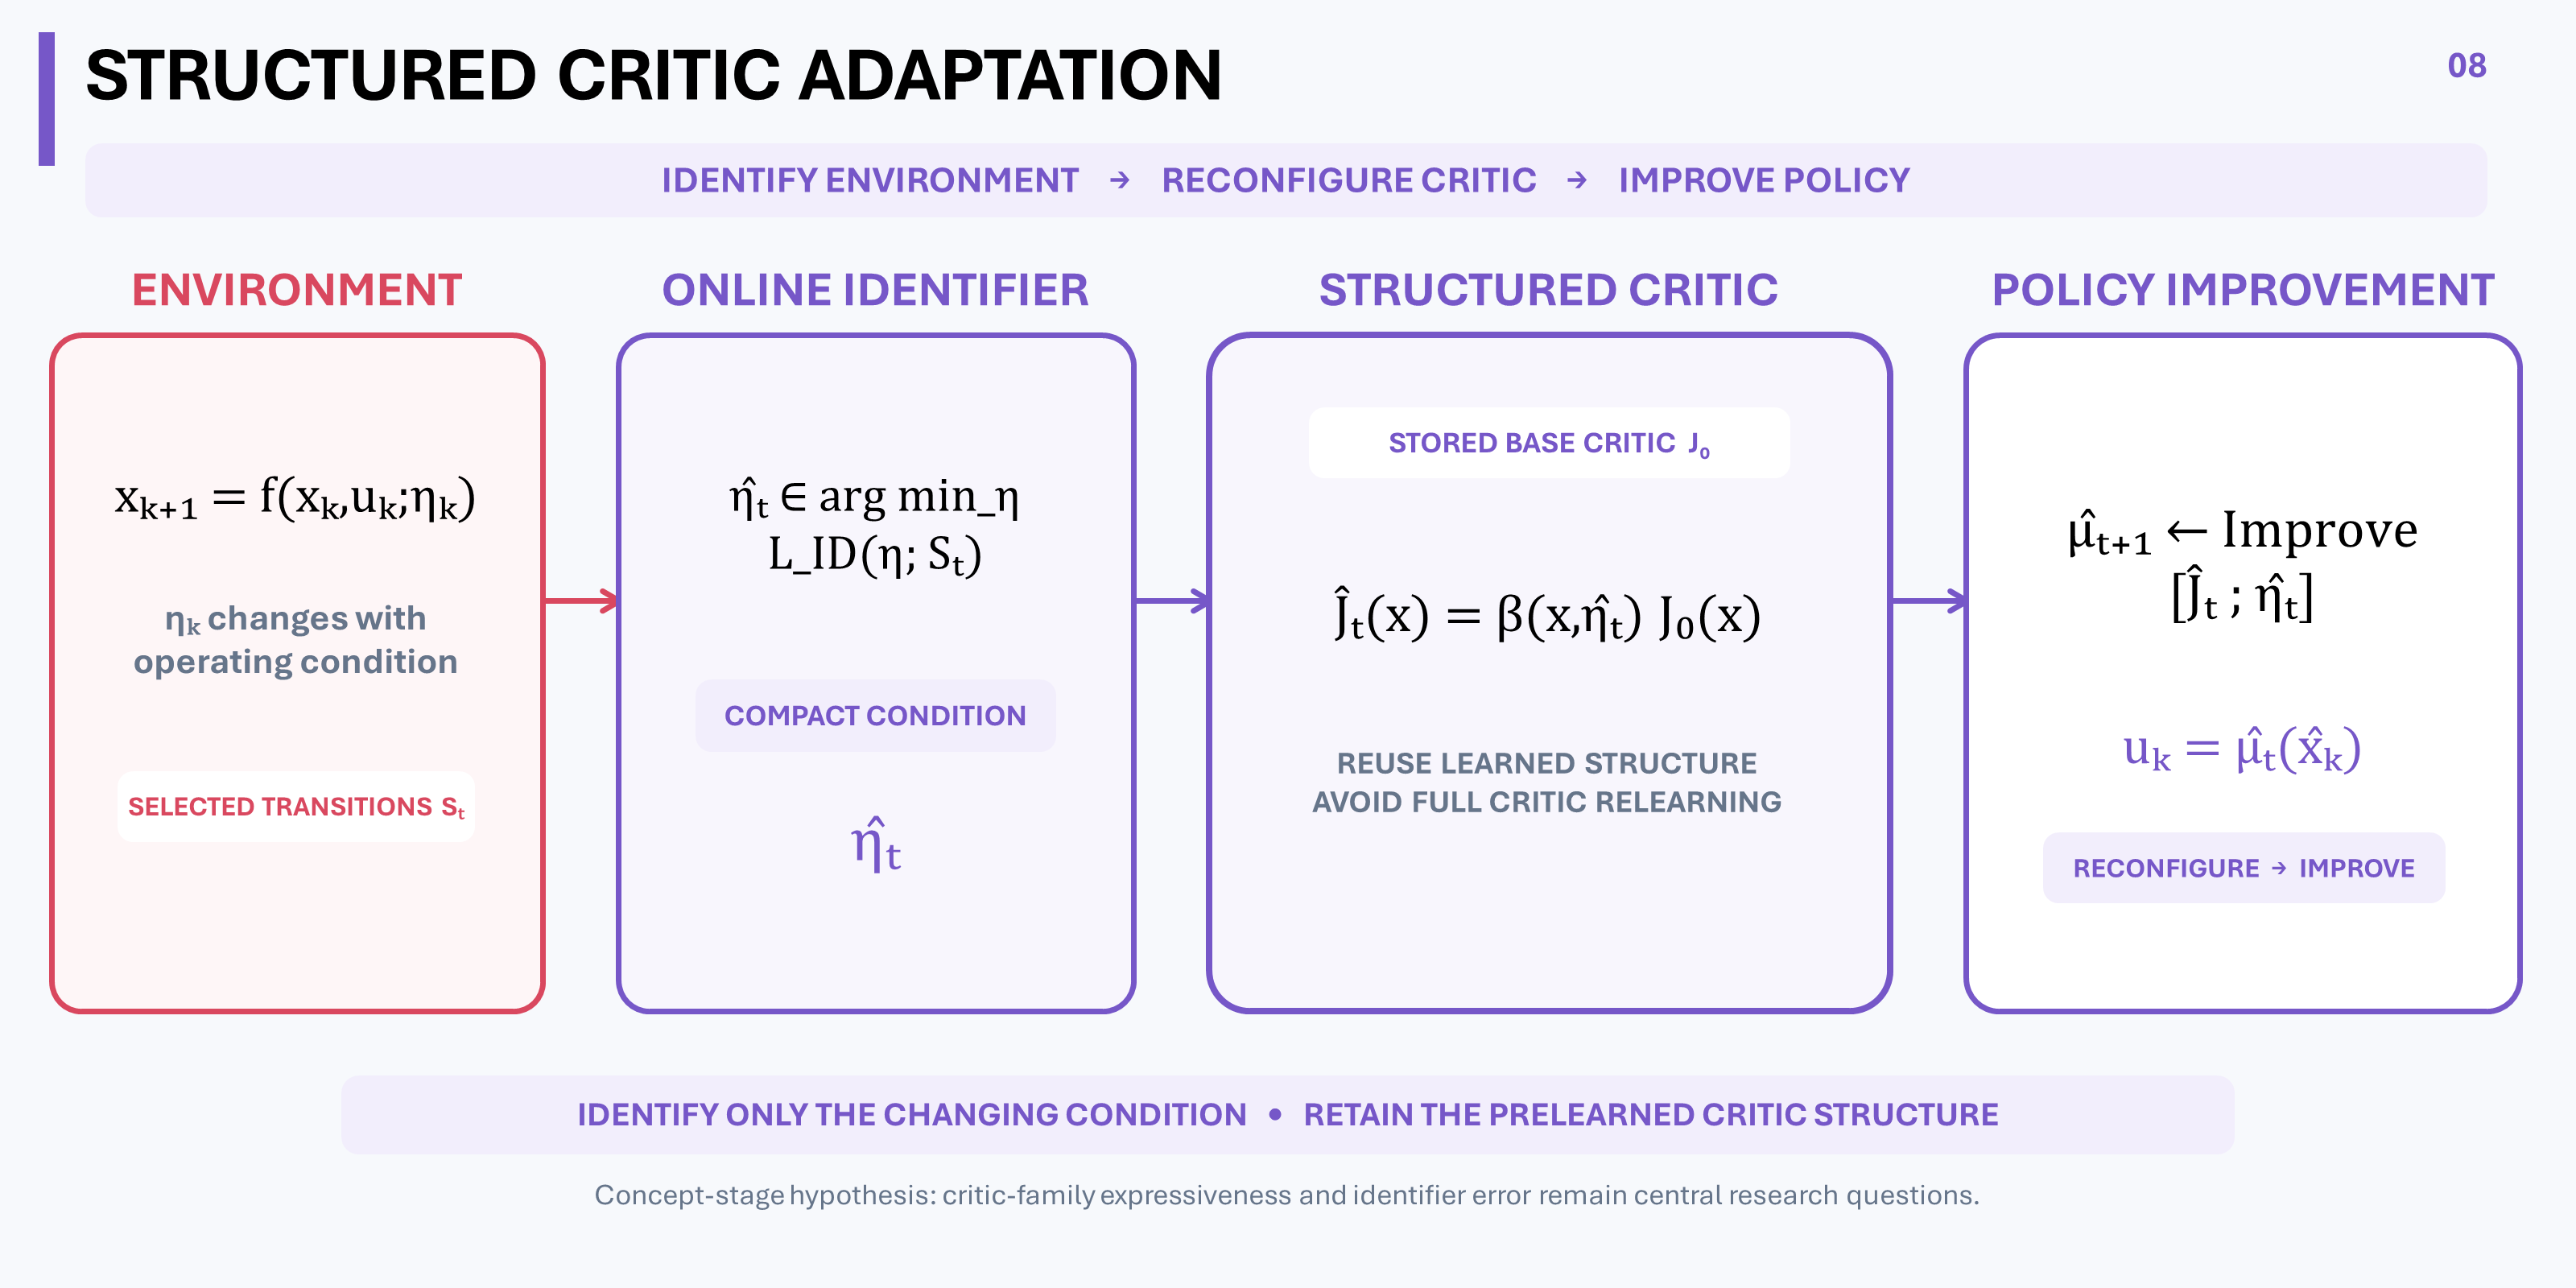
\includegraphics[width=\textwidth]{figures/08_structured_critic_adaptation.png}
  \caption{Selected transitions identify the environment, a learned structure reconfigures a stored critic, and the resulting critic improves the policy.}
\label{fig:}
\end{figure}

\nocite{*} % <------------ 인용있으면 삭제

Physical interaction is indexed by $k$, whereas identification and
policy updates are indexed by $t$. The environment parameter $\eta_k$ may vary
with physical conditions; $\widehat\eta_t$ is the estimate available at learner
update $t$, and $k(t)$ is the latest physical sample associated with that
update. Identification from a window assumes that $\eta_k$ is constant or
slowly varying over that window, or explicitly models its evolution.

\section{Problem definition}

\href{https://kaist-mic-lab.github.io/research/research_themes/00_online_learning_based_optimal_control/}{Online Learning-Based Optimal Control}
requires a critic appropriate to the current decision problem. Consider a
family of environments
\begin{equation}
  x_{k+1}=f(x_k,u_k;\eta_k)+w_k,
  \qquad
  y_k=h(x_k)+v_k,
\end{equation}
where $x_k$, $u_k$, and $y_k$ are the state, control input, and measurement;
$f$ and $h$ are the state-transition and measurement maps; and $w_k$ and
$v_k$ represent process and measurement uncertainty. The compact parameter
$\eta_k$ represents control-relevant changes in dynamics and, when declared,
in the stage cost $g$ or constraints. For notational simplicity, assume the
state is available; otherwise, an estimator supplies $\widehat x_k$.

Unless the evolution of $\eta_k$ is included in a Markov decision state, a
condition-specific critic $J_\eta$ below refers to the problem with $\eta$
fixed over its value horizon. Material variation over that horizon instead
requires a nonstationary formulation such as
\href{https://kaist-mic-lab.github.io/research/research_themes/04_nonstationary_infinite_horizon_ocp/}{Nonstationary Infinite-Horizon OCP}.

Let the transition record and the set selected at learner update $t$ be
\begin{equation}
  d_k=(x_k,u_k,g_k,x_{k+1}),
  \qquad
  g_k:=g(x_k,u_k;\eta_k),
  \qquad
  \mathcal S_t=\{d_k:k\in\mathcal I_t\},
\end{equation}
where $\mathcal I_t$ is the selected set of physical transition indices.
These recent transitions support online identification:
\begin{equation}
  \widehat\eta_t
  \in
  \operatorname*{arg\,min}_{\eta}
  \mathcal L_{\mathrm{id}}(\eta;\mathcal S_t).
\end{equation}

The loss $\mathcal L_{\mathrm{id}}$ must declare which effects identify
$\eta$: transition residuals when $\eta$ changes the dynamics, observed costs
when it changes the objective, or constraint/activity information when it
changes feasibility. A parameter that affects only an unobserved cost or
constraint cannot be identified from state transitions alone. The single
$\widehat\eta_t$ formulation assumes local constancy or sufficiently slow
variation over $\mathcal I_t$; otherwise, a trajectory-valued condition model
is required.

Let $J_0$ be a stored approximate base critic for a declared reference
condition $\eta_0$, and let $\beta_\omega(x,\eta)$ be a structural map learned
over representative conditions. The current critic is reconfigured as
\begin{equation}
  \widehat J_t(x):=\beta_\omega(x,\widehat\eta_t)J_0(x),
\end{equation}
and then used for policy improvement:
\begin{equation}
  \widehat\mu_{t+1}
  \leftarrow
  \operatorname{Improve}
  \!\left[\widehat J_t;\widehat\eta_t\right].
\end{equation}

The generic $\operatorname{Improve}$ operator may denote a declared
model-based Bellman improvement or a policy-network update. One-step lookahead
is therefore a possible implementation, not part of the Theme definition.
Here adaptation means reconfiguration through the identified condition, not
unrestricted online retraining of all critic parameters. The multiplicative
$\beta_\omega J_0$ form is the current schematic hypothesis; additive
corrections or critic-bank interpolation require separate definitions.

\section{Why this problem matters}

Direct adaptive-DP updates can repeatedly modify the full critic whenever the
operating condition changes. Such updates may fit the current condition while
overwriting behavior useful under earlier conditions, so a recurring
condition can require relearning.

If the environment family is organized by an identifiable parameter $\eta$,
a prelearned relation from $(x,\eta)$ to critic shape can reuse structure
across conditions. Online computation is then concentrated on estimating
$\eta$ and improving the policy from the reconfigured critic. This is a
conditional opportunity, not a guaranteed speedup: it depends on
identifiability, offline coverage, and the expressiveness of the critic
family.

\section{Key challenges}

\begin{itemize}
  \item \textbf{Environment representation and identification:}\\
  $\eta$ must
  capture control-relevant variation and be identifiable from the limited,
  policy-dependent data in $\mathcal S_t$.
  \item \textbf{Structured-family expressiveness:} the family
  $\beta_\omega(x,\eta)J_0(x)$ may be too restrictive, especially near zeros
  or sign changes of $J_0$.
  \item \textbf{Error propagation and changing conditions:} identification
  delay, structural approximation error, stale parameters, and model error
  perturb both the critic and the improved policy.
  \item \textbf{Bellman and closed-loop consistency:} a plausibly shaped
  critic is not automatically Bellman-consistent, stabilizing,
  constraint-satisfying, or reliable outside the representative offline
  conditions.
\end{itemize}

\section{A conventional approach --- direct critic adaptation}

A conventional adaptive-DP realization updates critic parameters directly
from recent data and then improves the policy:
\begin{equation}
  \begin{aligned}
    \theta_{t+1}
    &\approx
    \operatorname*{arg\,min}_{\theta}
    \mathcal L_{\mathrm{critic}}(\theta;\mathcal S_t),\\
    \widehat\mu_{t+1}
    &\leftarrow
    \operatorname{Improve}
    \!\left[\widehat J_{\theta_{t+1}}\right].
  \end{aligned}
\end{equation}

One representative choice for $\mathcal L_{\mathrm{critic}}$ is a sampled
one-step TD loss. Holding the target critic $\widehat J_{\bar\theta_t}$ fixed
during learner update $t$ and taking $0<\alpha<1$, define
\begin{equation}
  \begin{aligned}
    y_{k,t}^{\mathrm{TD}}
    &=g_k+\alpha\widehat J_{\bar\theta_t}(x_{k+1}),\\
    \mathcal L_{\mathrm{critic}}(\theta;\mathcal S_t)
    &=\frac{1}{|\mathcal S_t|}
    \sum_{k\in\mathcal I_t}
    \left(
    \widehat J_\theta(x_k)-y_{k,t}^{\mathrm{TD}}
    \right)^2.
  \end{aligned}
\end{equation}

This form evaluates the policy that generated the transitions, subject to the
usual on-policy or correction assumptions. If $\mathcal S_t$ mixes behavior
policies or materially different environment conditions, the window must be
restricted or an explicit off-policy/condition correction must be supplied.
If a model and action minimization are available, an empirical
Bellman-optimality target can be used instead. The selected critic loss and
its policy-evaluation or policy-improvement role must be declared.

This can track the currently visited condition, but it does not explicitly
preserve a reusable relation between the environment parameter and critic
shape. Under limited data, it may repeatedly overwrite and relearn critic
behavior as conditions change. This is a baseline mechanism, not a claim that
every direct critic update necessarily forgets.

\section{Candidate direction --- identifier-conditioned critic reconfiguration}

Offline, suppose approximate critics $\{\widehat J^{(m)}\}$ are available for
representative conditions $\{\eta^{(m)}\}$ under a common state representation,
objective, discount, and solution concept. In the optimal-control case,
$\widehat J^{(m)}\approx J_{\eta^{(m)}}^\star$, where $J_\eta^\star$ denotes
the optimal critic for the fixed-condition problem. Hold the reference critic
$J_0$ fixed and fit the structural map through
\begin{equation}
  \omega^\dagger
  \in
  \operatorname*{arg\,min}_{\omega}
  \sum_m
  \left\|
  \widehat J^{(m)}(\cdot)
  -
  \beta_\omega(\cdot,\eta^{(m)})J_0(\cdot)
  \right\|_{\nu_m}^{2},
\end{equation}
where $\nu_m$ is a declared weighting distribution or measure over
control-relevant states and
$\|e\|_{\nu_m}^2:=\int |e(x)|^2\,d\nu_m(x)$. If $J_0$ is to be learned jointly
instead, it must appear as an optimization variable and a normalization is
needed to remove the scaling ambiguity between $J_0$ and $\beta_\omega$.
Online operation then follows
\begin{equation}
  \begin{aligned}
    \mathcal S_t
    &\xrightarrow{\text{online identification}}
    \widehat\eta_t,\\
    \widehat J_t(x)
    &=\beta_{\omega^\dagger}(x,\widehat\eta_t)J_0(x),\\
    \widehat\mu_{t+1}
    &\leftarrow
    \operatorname{Improve}
    \!\left[\widehat J_t;\widehat\eta_t\right].
  \end{aligned}
\end{equation}

A useful diagnostic, rather than a guarantee, separates two critic errors.
For compactness, let $\eta_t:=\eta_{k(t)}$ denote the physical environment
condition associated with learner update $t$. The norm below must use the same
declared control-relevant domain or measure for all terms:
\begin{equation}
  \begin{aligned}
    \left\|\widehat J_t-J_{\eta_t}^{\star}\right\|
    \le {}&
    \left\|
    \beta_{\omega^\dagger}(\cdot,\widehat\eta_t)J_0
    -\beta_{\omega^\dagger}(\cdot,\eta_t)J_0
    \right\|\\
    &+
    \left\|
    \beta_{\omega^\dagger}(\cdot,\eta_t)J_0
    -J_{\eta_t}^{\star}
    \right\|.
  \end{aligned}
\end{equation}

The first term audits sensitivity to identification error; the second audits
the structured critic family. Policy-improvement and model errors remain
additional. Research questions include how to select $\eta$, how to learn
$J_0$ and $\beta_\omega$, when an additive or critic-bank structure is more
appropriate, how to represent uncertainty in $\widehat\eta_t$, and when to
reject reconfiguration in favor of a safe fallback.

Future evidence should compare a fixed $J_0$, direct critic adaptation, the
structured method with oracle $\eta$, and the method with estimated $\eta$.
Relevant metrics include identification error and delay, critic and Bellman
error, closed-loop performance, violations, update latency, memory, and
return-to-prior-condition performance under abrupt, gradual, recurring, and
held-out conditions.

\section{Application domains}

\begin{itemize}
  \item \textbf{Mobility controllers under changing mass, load, road--tire
  condition, temperature, or component aging:} estimate a compact condition
  parameter and reconfigure a stored critic so recurring operating regimes can
  reuse previously learned long-run control structure.
  \item \textbf{Electric-drive and mechatronic control} with compact
  identifiable plant parameters, such as resistance, inertia, friction, or
  load, that can condition a reusable critic family and its subsequent policy
  improvement.
  \item \textbf{Systems that revisit a finite or smoothly parameterized
  environment family:} recover or interpolate an appropriate critic when a
  known condition returns, rather than relearning the full value function from
  the latest trajectory. The benefit depends on identification quality and
  offline coverage of that environment family.
\end{itemize}

\end{document}
